\subsubsection{Recherche zu Risiko R16: Blendung der Kamera durch Reflexionen}
Um Reflexionen zu reduzieren, kann im Fotografikbereich mit Polarisationsfiltern gearbeitet werden, die nur Licht mit einer gewissen Polarisierung durchlassen. Mit Hilfe eines solchen Polarisationsfilters wurden Tests gemacht, um zu sehen, inwiefern die Reflexionen tatsächlich reduziert werden können. Dabei wurde darauf geachtet, dieselben Kamera-Einstellungen mit und ohne Polarisationsfilter zu verwenden.

\begin{table}[h!]
    \centering
    \begin{tabular}{|c|c|}
        \hline
        \parbox[c][1cm][c]{3cm}{\centering Ohne Polarisationsfilter} &
        \parbox[c][1cm][c]{3cm}{\centering Mit Polarisationsfilter} \\
        \hline
        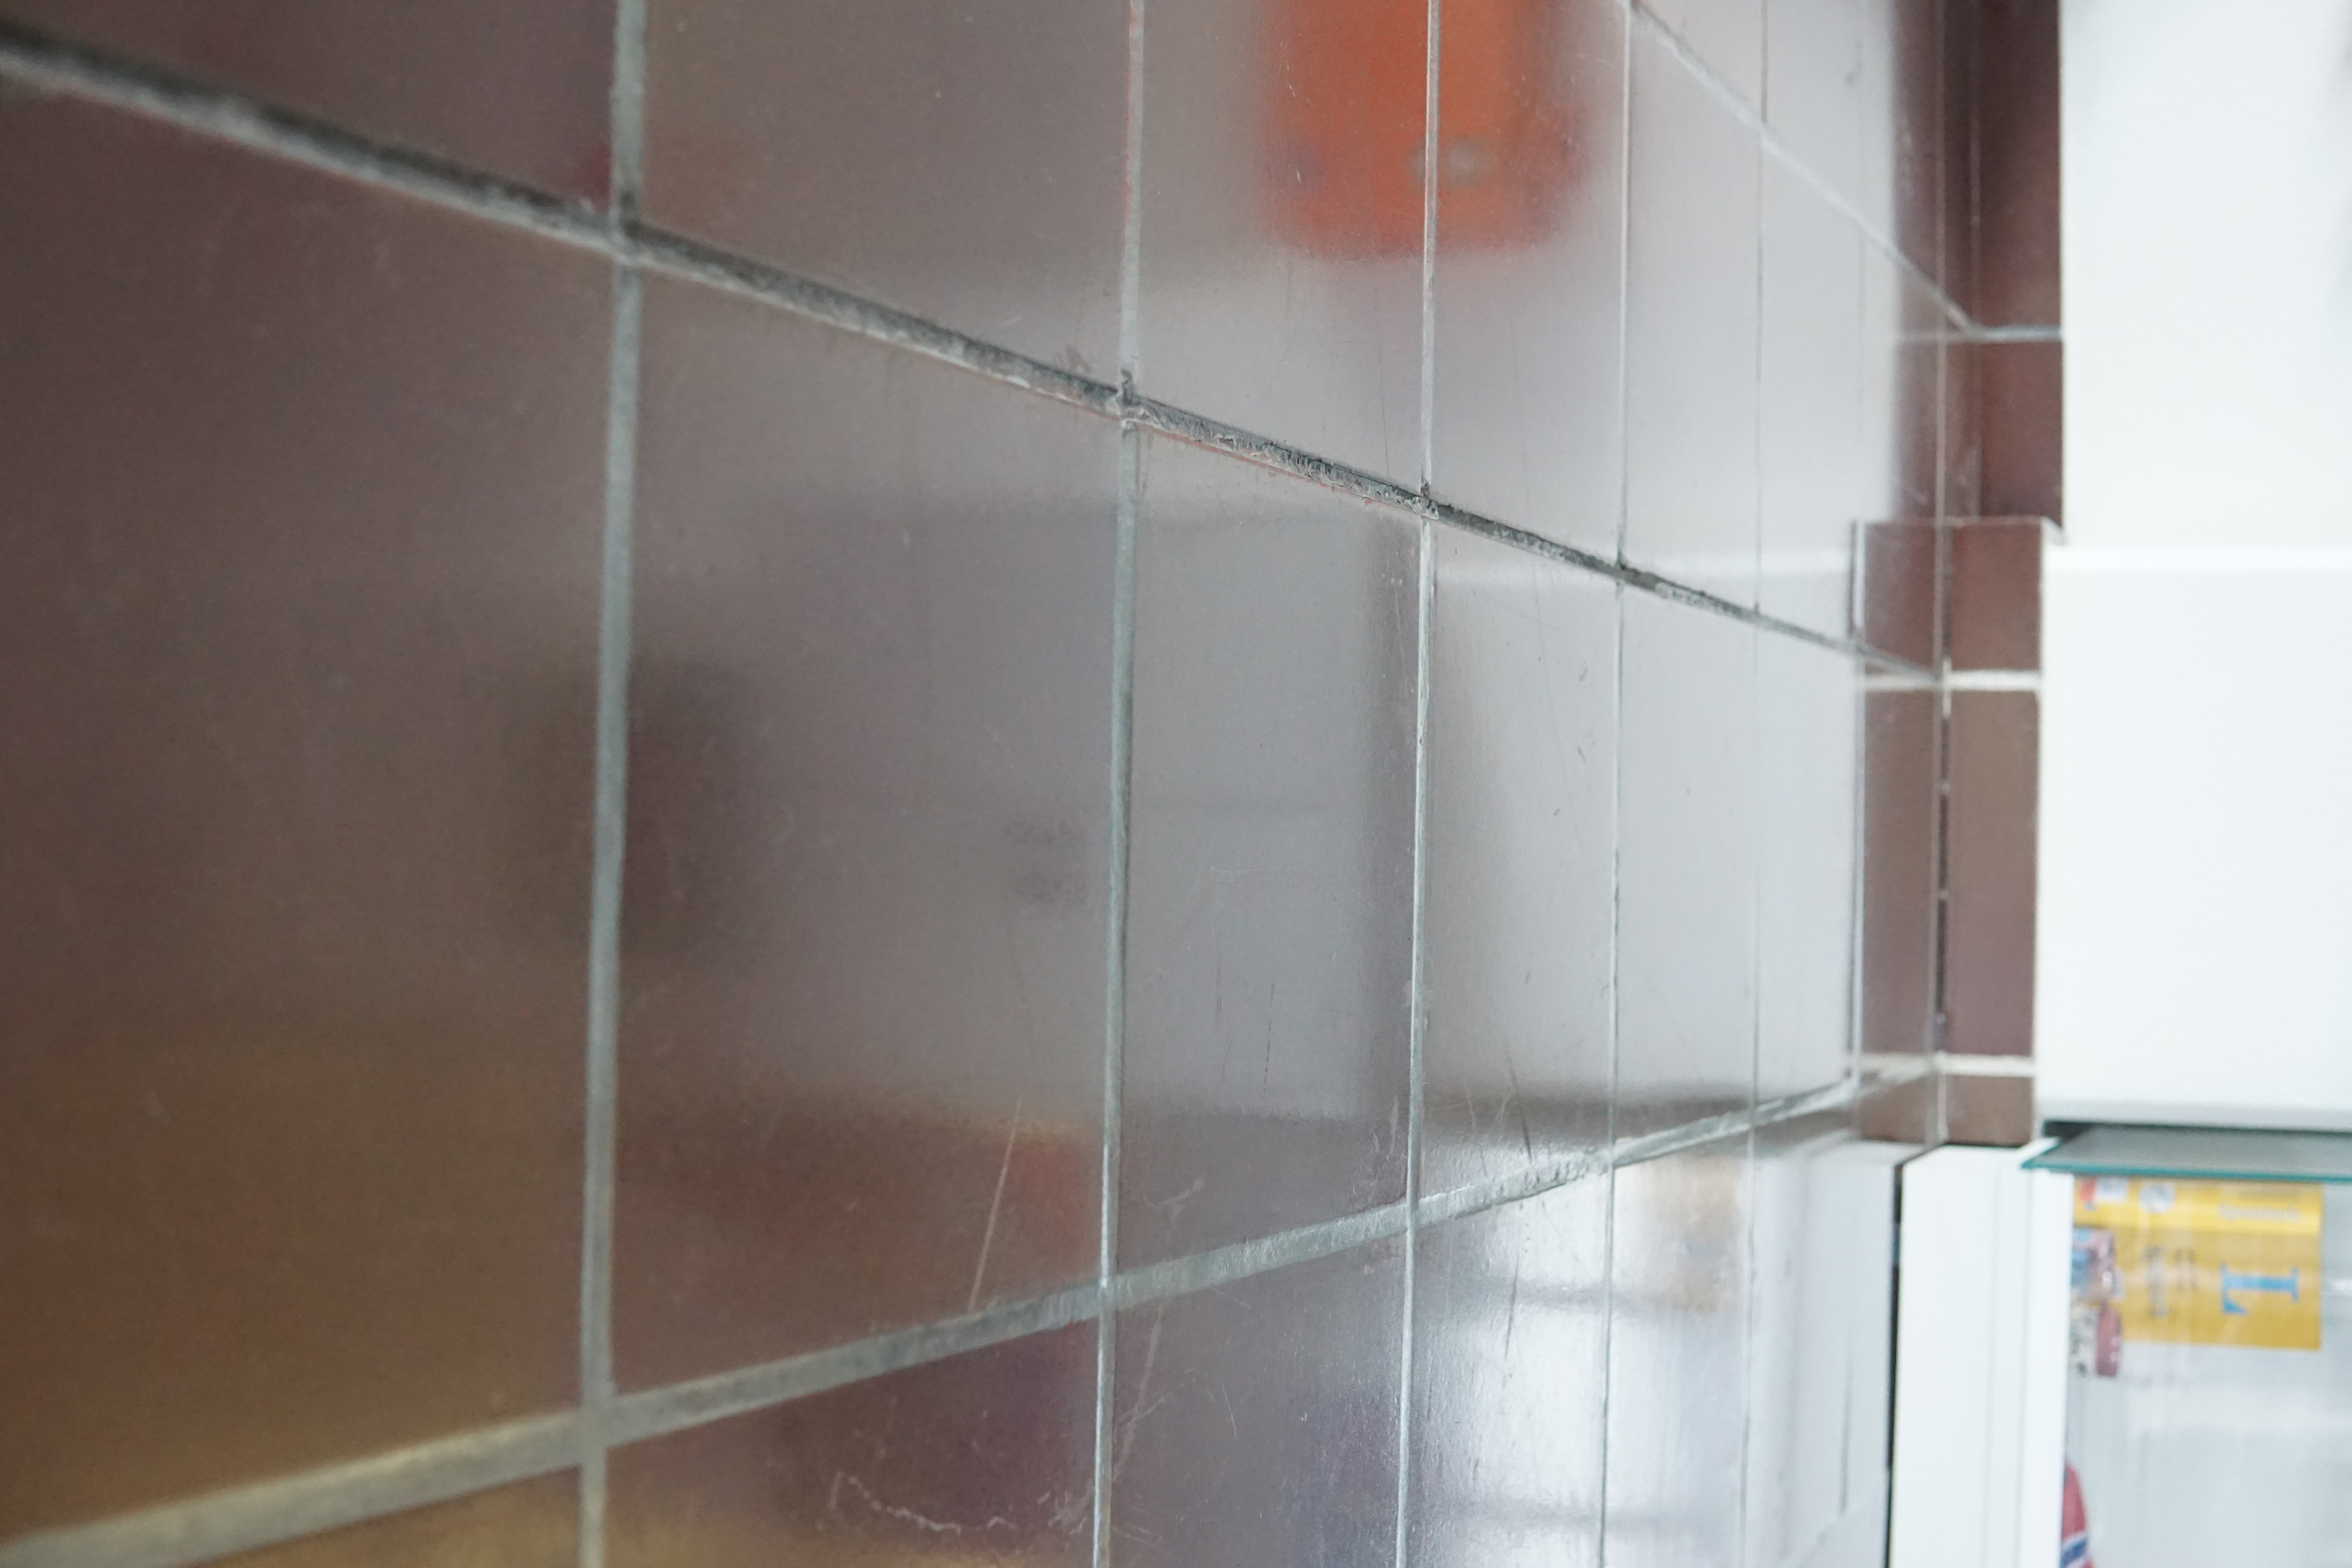
\includegraphics[width=6cm,angle=90,origin=c]{img/polarisierungsfilter/pol4_n.jpg} & 
        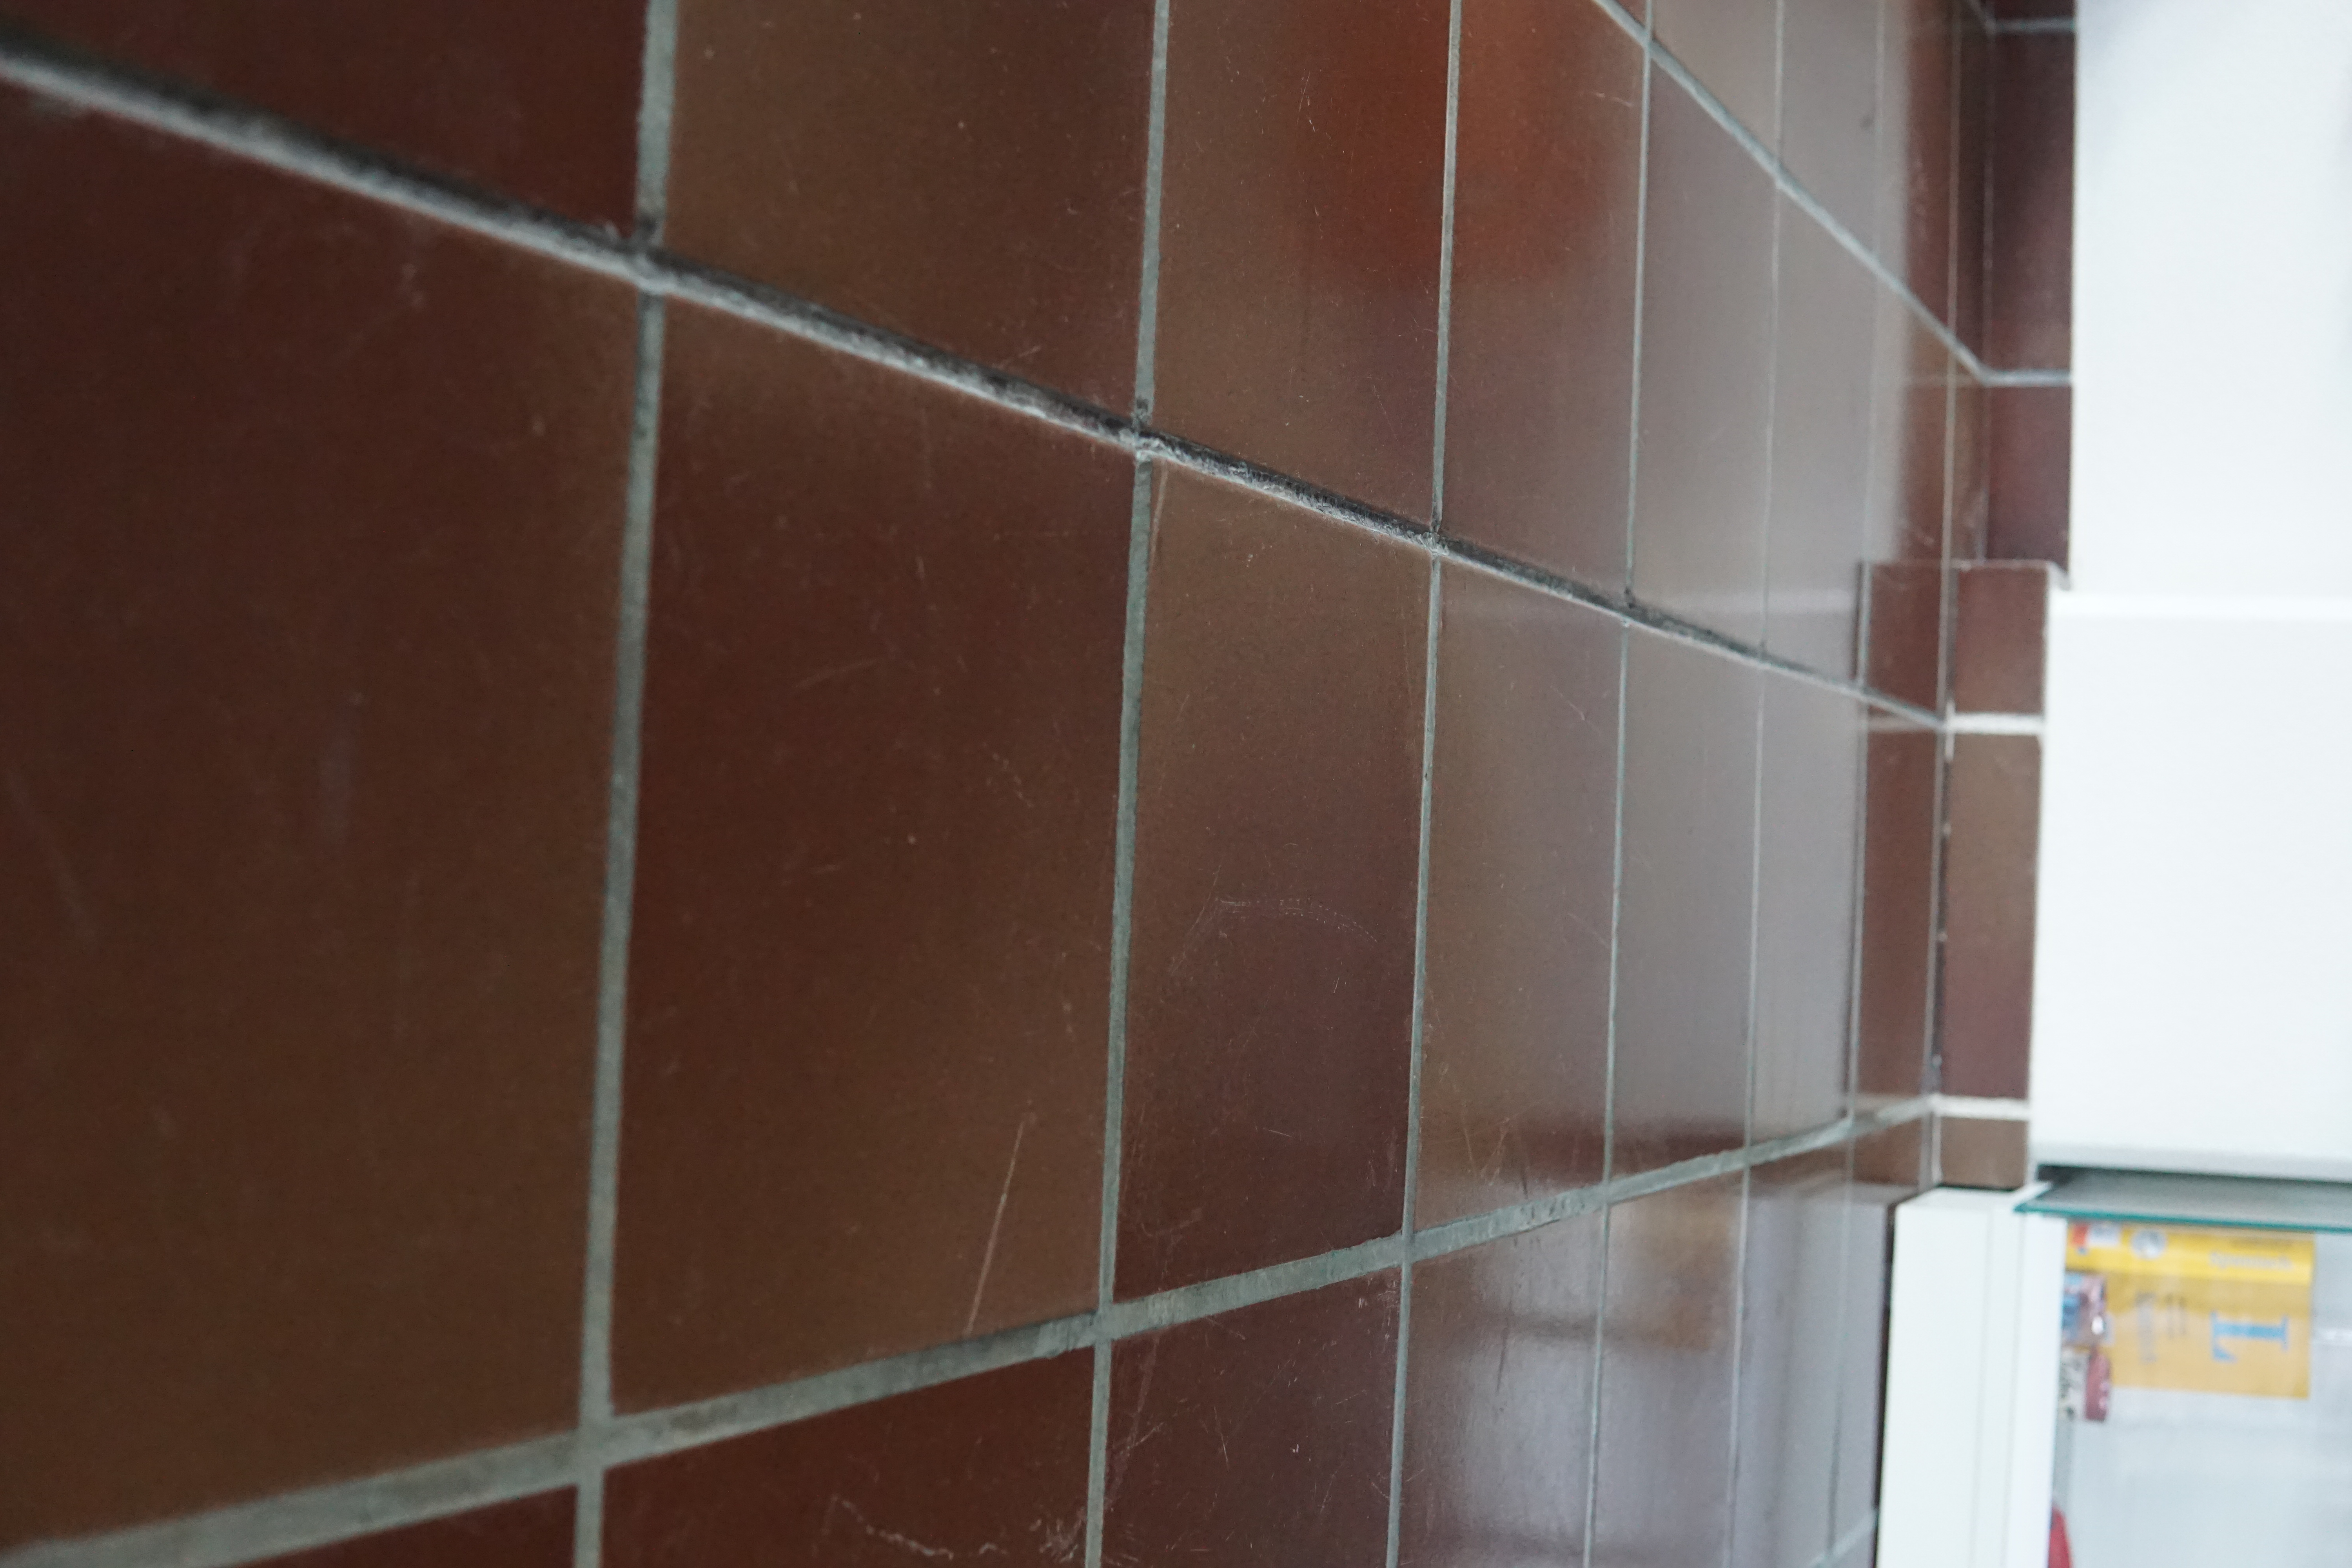
\includegraphics[width=6cm,angle=90,origin=c]{img/polarisierungsfilter/pol4_j.jpg}  \\
        \hline 
        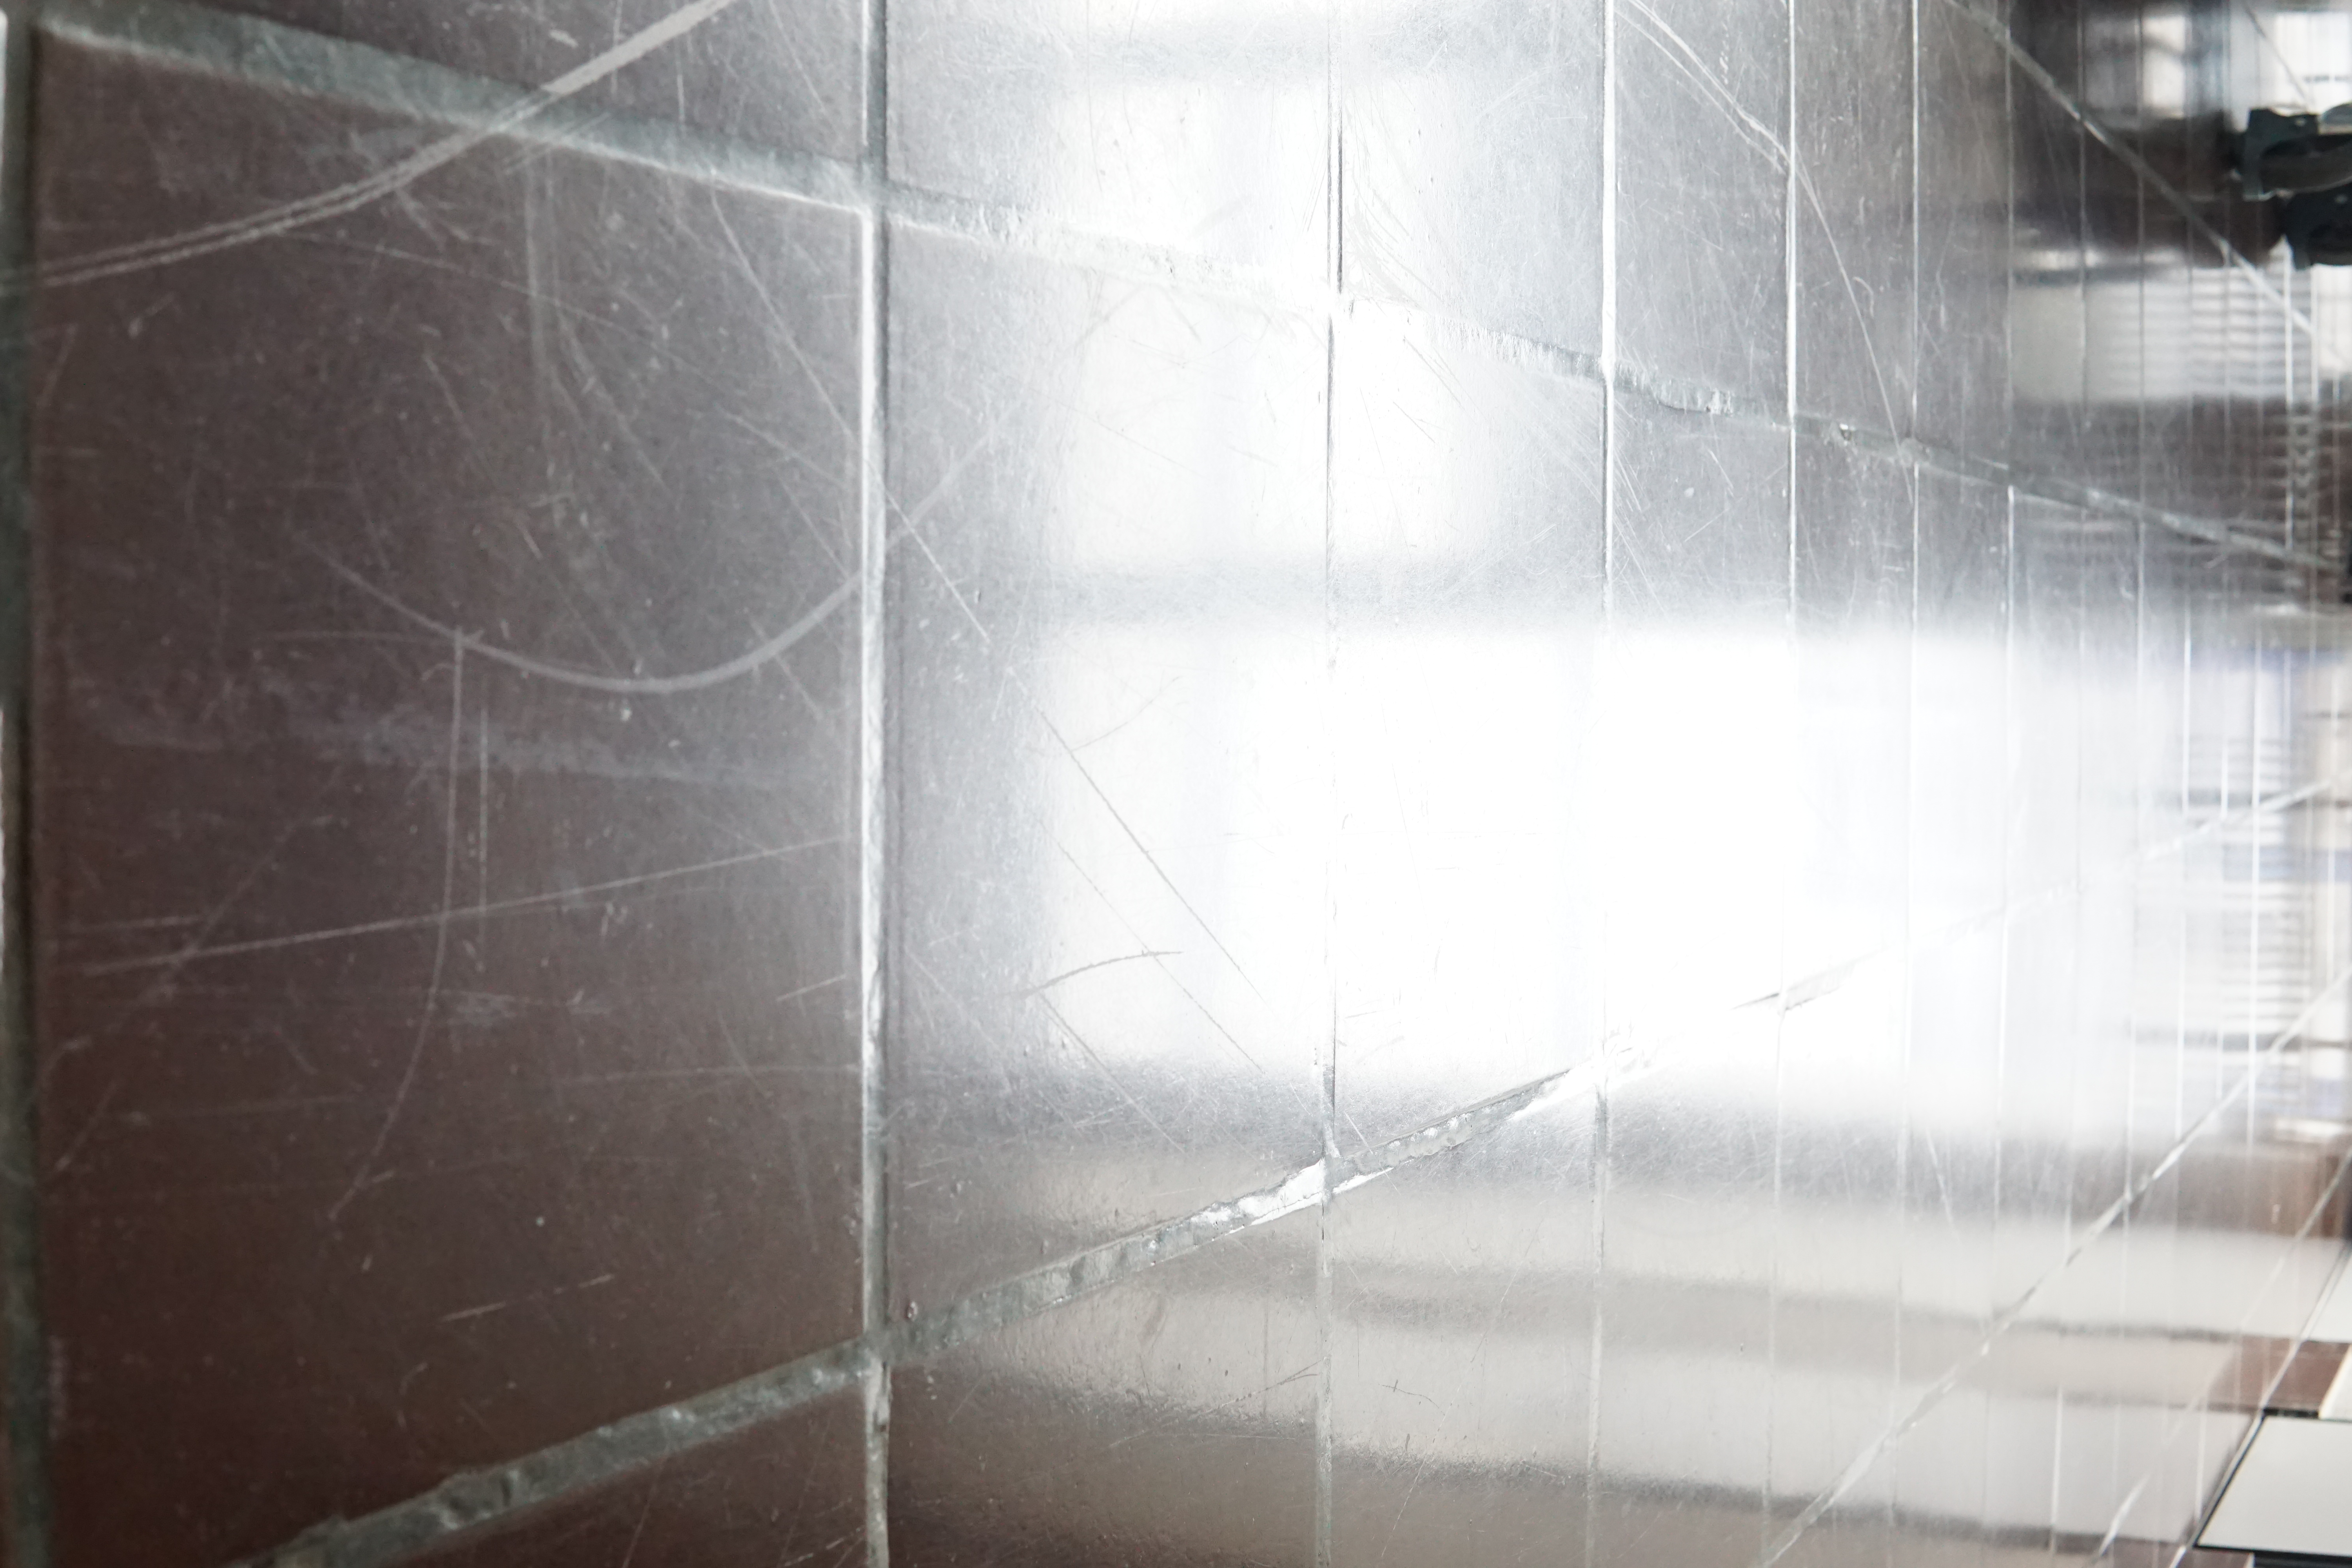
\includegraphics[width=6cm,angle=90,origin=c]{img/polarisierungsfilter/pol5_n.jpg} & 
        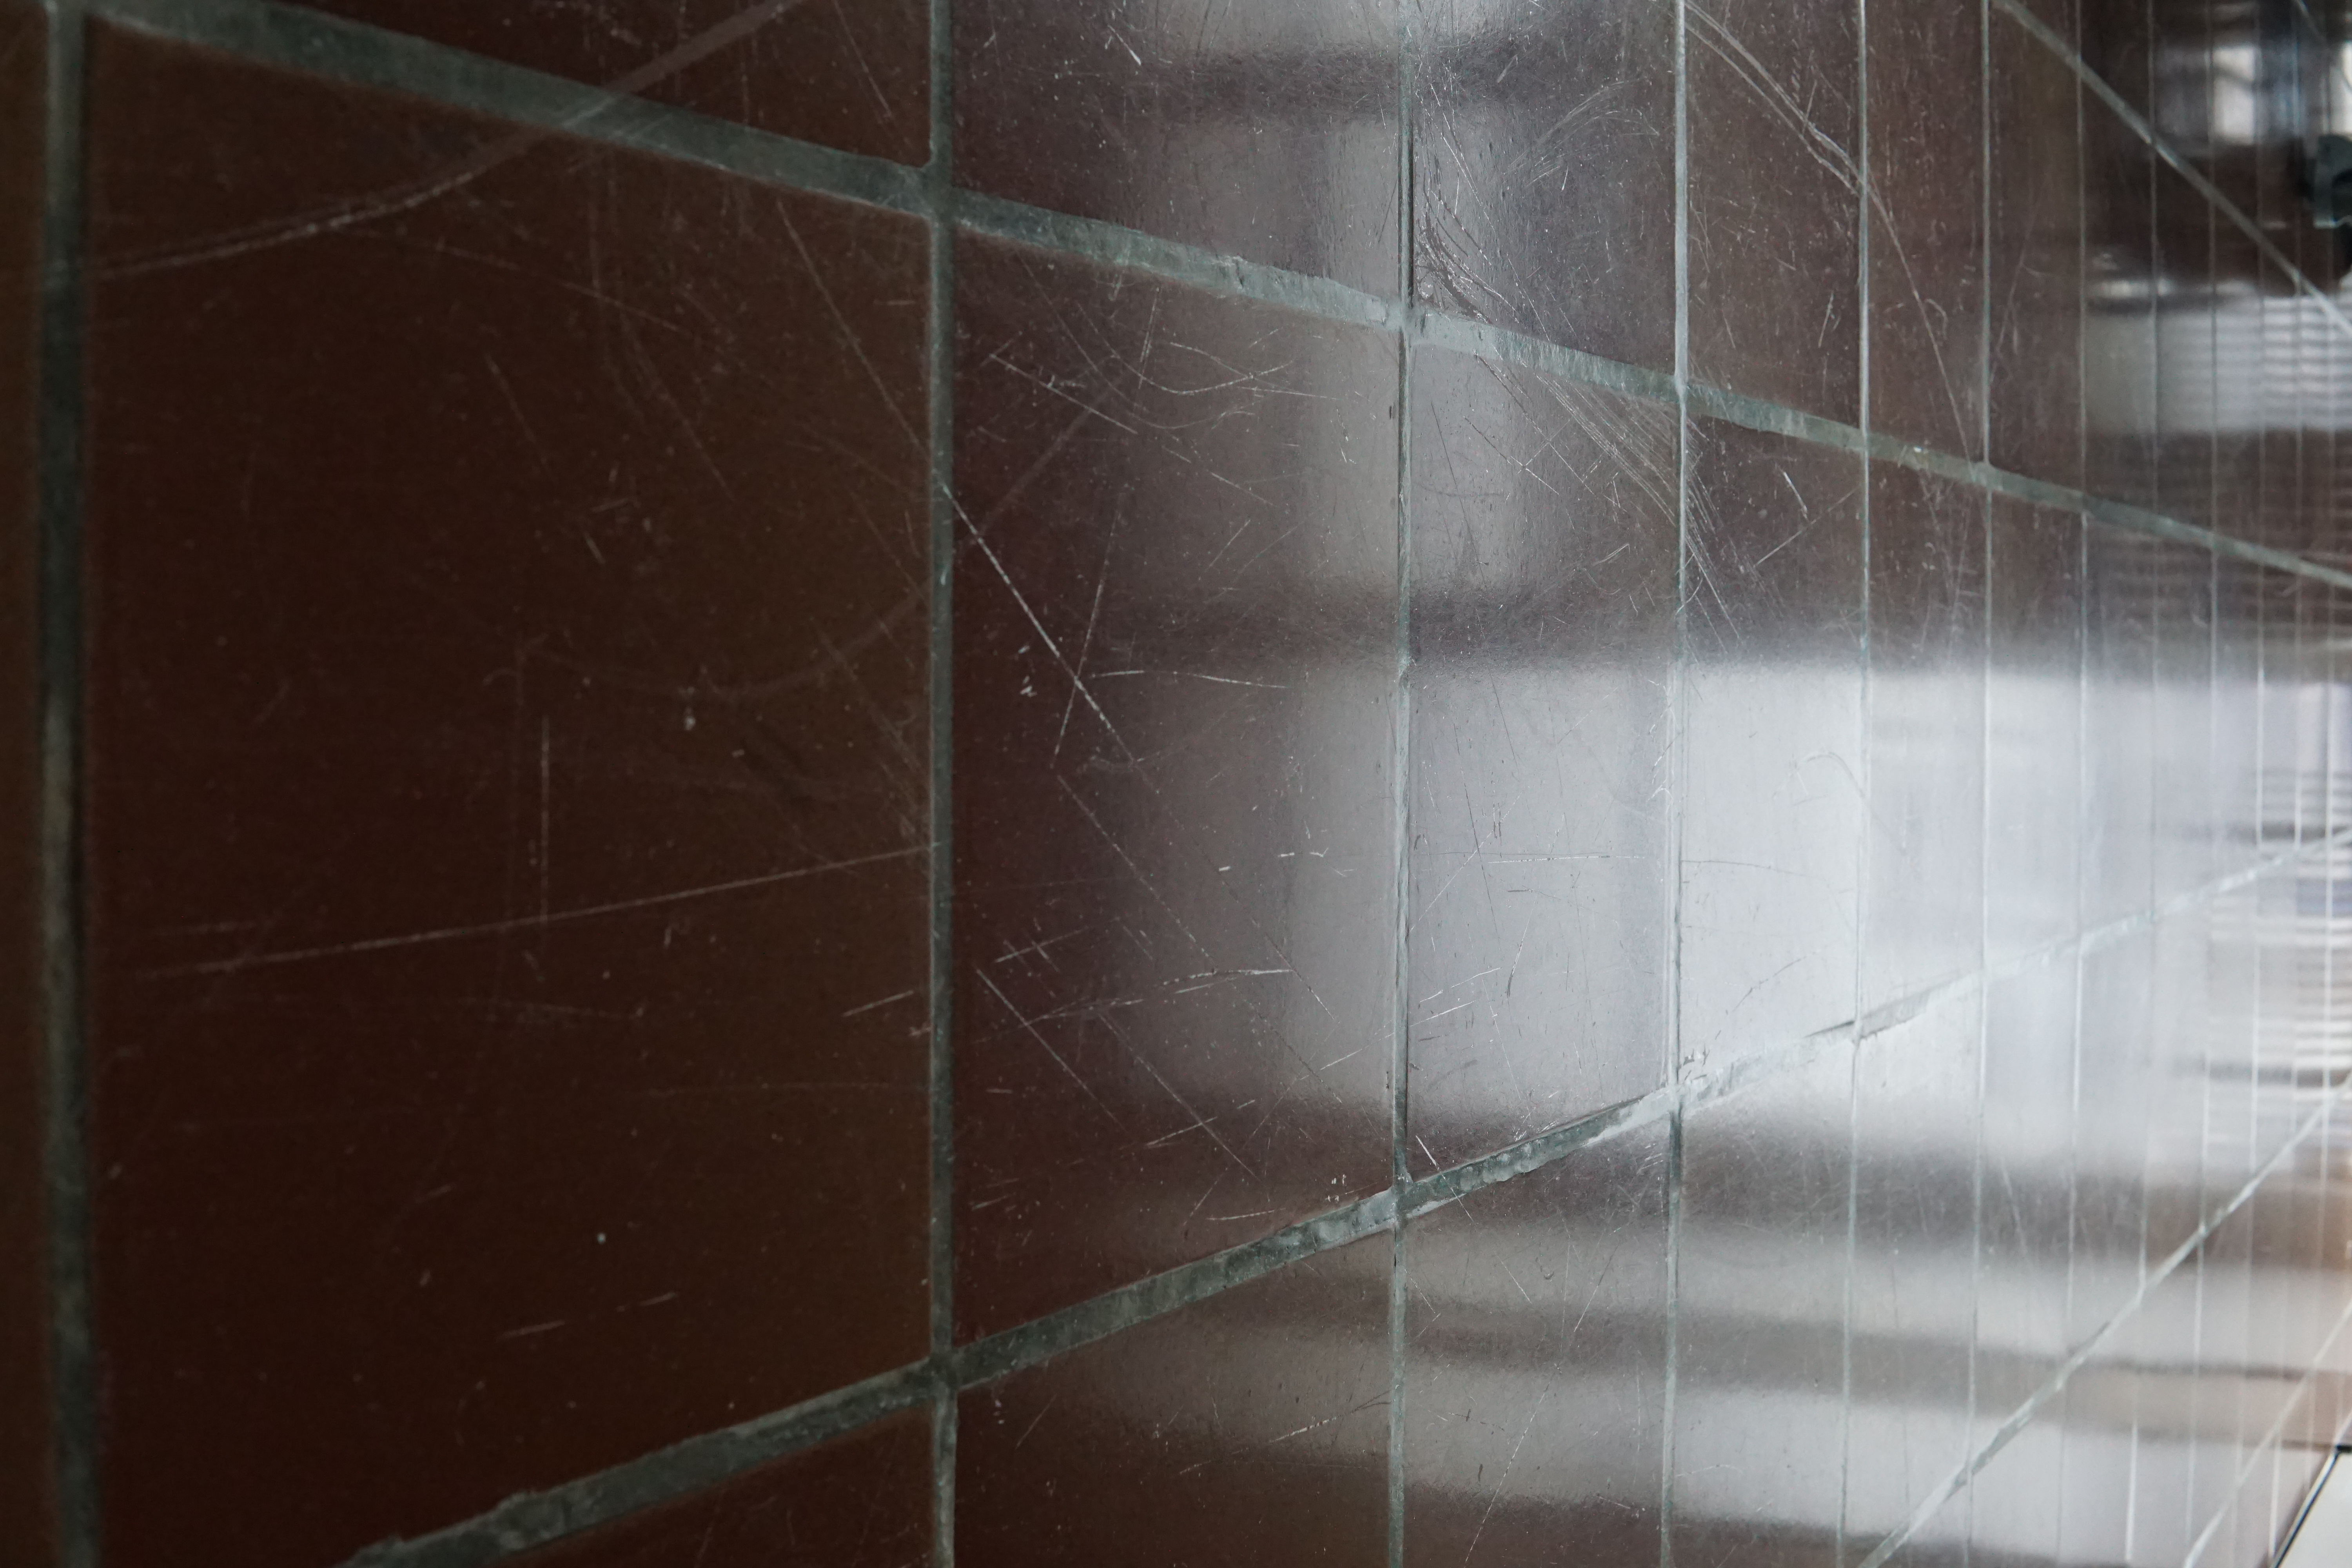
\includegraphics[width=6cm,angle=90,origin=c]{img/polarisierungsfilter/pol5_j.jpg} \\
        \hline
    \end{tabular}
    \caption{Vergleich Polarisationsfilter}
\end{table}

Die Resultate sind eindeutig. Bei gleichen Kamera-Einstellungen reduziert ein Polarisationsfilter die Reflexionen auf den Bodenplatten deutlich.